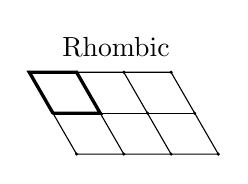
\begin{tikzpicture}[scale=0.2]



%draw the rhombic lattice
\coordinate (rhombic) at (2.5,5.6);
\node [above] at (rhombic) {Rhombic};

\draw (0,0) -- ++(0:9) -- ++(120:6) -- ++(180:9) -- cycle;
\draw (3,0) -- ++(120:6);
\draw (6,0) -- ++(120:6);
\draw (0,0) ++(120:3) -- ++(0:9);

\draw [very thick] (0,0) ++(120:3) -- ++(0:3) -- ++(120:3) -- ++(180:3) -- ++(300:3);

\draw (0,0) coordinate(r00) ++(0:3) coordinate(r01) ++(0:3) coordinate(r02) ++(0:3) coordinate(r03) ++(120:3) coordinate(r13) ++(180:3) coordinate(r12) ++(180:3) coordinate(r11) ++(180:3) coordinate(r10) ++(120:3)  coordinate(r20) ++(0:3) coordinate(r21) ++(0:3) coordinate(r22) ++(0:3) coordinate(r23);

\filldraw[fill=black, draw=black] (r00) circle (0.06);
\filldraw[fill=black, draw=black] (r01) circle (0.06);
\filldraw[fill=black, draw=black] (r02) circle (0.06);
\filldraw[fill=black, draw=black] (r03) circle (0.06);
\filldraw[fill=black, draw=black] (r10) circle (0.06);
\filldraw[fill=black, draw=black] (r11) circle (0.06);
\filldraw[fill=black, draw=black] (r12) circle (0.06);
\filldraw[fill=black, draw=black] (r13) circle (0.06);
\filldraw[fill=black, draw=black] (r20) circle (0.06);
\filldraw[fill=black, draw=black] (r21) circle (0.06);
\filldraw[fill=black, draw=black] (r22) circle (0.06);
\filldraw[fill=black, draw=black] (r23) circle (0.06);

\end{tikzpicture}

